\documentclass[10pt]{standalone}
\usepackage{tikz}
\usetikzlibrary{patterns}
\usepackage{pgfplots}
\usepackage{ifthen}
\usetikzlibrary{decorations.markings, calc}




\begin{document}
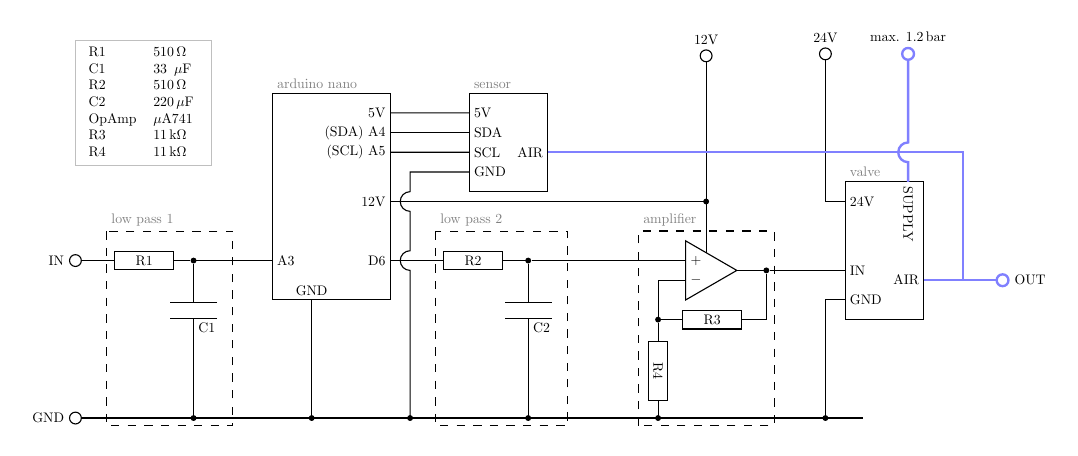
\begin{tikzpicture}[
scale = .5,
connect/.style={circle, fill=black, inner sep=0pt, minimum height=.75mm},
outerconnect/.style={circle, fill=white, draw, inner sep=0pt, minimum height=1.5mm},
fontnode/.style={scale=.5},
resistor/.style={sloped, scale=.5, fill=white!50, minimum width=1.5cm, draw},
fluid/.style={line width=.3mm, blue!50},
capacityLine/.style 2 args ={
    postaction={decorate,
        decoration={markings, mark= at position #1 with
           {\fill[white] (-0.1,-0.3) rectangle (0.1,0.3);
            \draw (-0.1,0.3) -- (-0.1,-0.3) (0.1,0.3) -- (0.1,-0.3)node[midway, anchor=north west, scale=.5]{#2};}}}}
]


%%%% GND 

\draw[] (-1,-8)coordinate(G)node[outerconnect](GND){}--++(20,0);
\path (GND.west)node[left, fontnode]{GND};

\path (-1,0) node[fontnode, right, align=left, draw=gray!50]{
\begin{tabular}{ll}
R1 & 510\,$\Omega$ \\
C1 & 33 \,$\mu$F \\
R2 & 510\,$\Omega$ \\
C2 & 220\,$\mu$F \\
OpAmp & $\mu$A741 \\
R3 & 11\,k$\Omega$ \\
R4 & 11\,k$\Omega$ \\
\end{tabular}
};



%%%% ARDUINO

\path (4,0)coordinate(Ard);

\draw (Ard)--++(0,-4)coordinate(A3)node[right, fontnode]{A3}--++(0,-1)--++(1,0)coordinate(AGND)node[above, fontnode]{GND}--++(2,0)coordinate(ArdBR)--++(0,1)coordinate(D6)node[left, fontnode]{D6}--++(0,1.5)coordinate(A12V)node[left, fontnode]{12V}--++(0,1.25)coordinate(A5)node[left, fontnode]{(SCL) A5} --++(0,.5)coordinate(A4)node[left, fontnode]{(SDA) A4}--++(0,.5)coordinate(A5V)node[left, fontnode]{5V}--++(0,.5)--++(-3,0)coordinate(Ard)--cycle;
\path (AGND) |- (G)coordinate[midway] (x);
\draw (AGND)--(x) node[connect]{};

\path (Ard)node[above right, fontnode, gray]{arduino nano};

%% LP IN
\draw (A3)--++(-2,0)node[connect](c1){};
\path (c1) |- (G)coordinate[midway] (x);
\draw[capacityLine={.3}{C1}] (c1)--(x) node[connect](C1){};
\draw (c1)--++(-3,0)node[pos=.4, resistor](r1){R1}node[outerconnect](IN){};
\draw[dashed] (r1.north west)++(-.2, .5)node[above right, fontnode, gray]{low pass 1}rectangle ($(C1)+(1,-.2)$);

\path (IN.west)node[left, fontnode]{IN};

%% LP OUT
\draw (D6)--++(3.5,0)node[pos=.6, resistor](r2){R2}node[connect](c2){};
\path (c2) |- (G)coordinate[midway] (x);
\draw[capacityLine={.3}{C2}] (c2)--(x) node[connect](C2){};
\draw[dashed] (r2.north west)++(-.2, .5)node[above right, fontnode, gray]{low pass 2}rectangle ($(C2)+(1,-.2)$);

%% OPAMP
\draw (c2)--++(4,0)coordinate(OPAMP1);
\draw (OPAMP1)node[right, fontnode]{$+$}--++(0,-.5)coordinate(OPAMP2)node[right, fontnode]{$-$}--++(0,-.5)--++(30:1.5)coordinate(OPAMP3)--++(150:1.5)coordinate[pos=.6](OPAMP4)--cycle;
\draw(OPAMP3)--++(.75,0)node[connect](c3){};
\draw (c3)--++(0,-1.25)--++(-2.75,0)node[resistor, midway]{R3}node[connect](c4){}|-(OPAMP2);
\path (c4) |- (G)coordinate[midway] (x);
\draw (c4)--(x)node[resistor, midway]{R4} node[connect](C4){};
\draw[dashed] (C4)++(-.5,-.2)|- ($(c3)+(.2,1)$)node[midway, above right, fontnode, gray]{amplifier}|-cycle;
\draw (OPAMP4)--++(0,5)node[outerconnect](12V){};
\path (12V.north) node[above, fontnode]{12V};

\path (A12V)-|(OPAMP4)coordinate[midway](x);
\draw (A12V)--(x)node[connect]{};



%% VALVE
\draw (c3)--++(2,0)coordinate(V1)node[right, fontnode]{IN}--++(0,1.75)coordinate(V24V)node[right, fontnode]{24V}--++(0,.5)coordinate(Valve)-|++(2,-2.5)coordinate[pos=.4](VIN)node[pos=.4, right, rotate=-90, fontnode]{SUPPLY}coordinate(V3)node[left, fontnode]{AIR}|-++(-2,-1)--++(0,.5)coordinate(V4)node[right, fontnode]{GND}--++(0,1);
\path (V4)++(-.5,0) |- (G)coordinate[midway] (x);
\draw (V4)--++(-.5,0)--(x)node[connect]{};
\path (Valve)node[above right, fontnode, gray]{valve};
\draw (V24V)--++(-.5,0)--++(0,3.75)node[outerconnect](24V){};
\path (24V.north)node[above, fontnode]{24V};

\draw[fluid] (VIN)--++(0,.5)arc(270:90:.25)--++(0,2.25)node[outerconnect](AIRIN){};
\path (AIRIN.north)node[above, fontnode]{max. 1.2\,bar};
%% PSENS

\draw (A4)--++(2,0)node[right, fontnode]{SDA}--++(0,-.5)coordinate(PSens2)node[right, fontnode]{SCL}--++(0,-.5)coordinate(PSens3)node[right, fontnode]{GND}--++(0,-.5)--++(2,0)--++(0,1)coordinate(PSens4)node[left, fontnode]{AIR}--++(0,1.5)--++(-2,0)coordinate(PSens)--++(0,-.5)coordinate(PSens5)node[right, fontnode]{5V}--++(0,-.5);
\draw (A5)--(PSens2);
\draw (A5V)--(PSens5);
\path (PSens3)++(-1.5,0) |- (G)coordinate[midway] (x);
\draw (PSens3)--++(-1.5,0)--++(0,-.5)arc(90:270:.25)--++(0,-1)arc(90:270:.25)--(x)node[connect]{};
\path (PSens)node[above right, fontnode, gray]{sensor};


%% Fluid

\draw[fluid] (V3)--++(1,0)coordinate(a1)|-(PSens4);
\draw[fluid] (a1)--++(1,0)node[outerconnect](AIR){};
\path (AIR.east)node[right, fontnode]{OUT};

\end{tikzpicture}
\end{document}